%!TEX root = ../../thesis.tex

\subsection{The anatomy of an event}

\ac{MC} event generators provide fully-exclusive hadron-level simulation of \pp collision 
events at the \acs{LHC} \cite{MCnet:general}. \Figure~\ref{fig:mcevent} shows how event 
generation is factorised into several components, each describing a certain regime of 
momentum transfer.

\begin{figure}[b]
	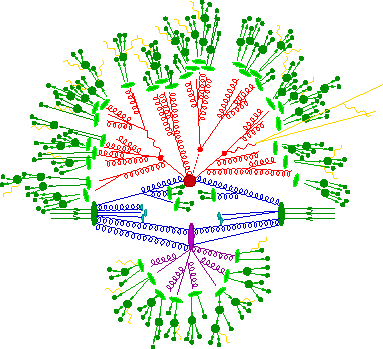
\includegraphics[width=\mediumfigwidth]{tex/tools/event}
	\caption{Schematic diagram of a simulated \ttH event, showing how factorisation allows 
	the physics at different scales of momentum transfer $Q$ to be treated independently 
	\cite{MCnet:MatchingLectures}.
	At high-$Q$ is the hard scatter (red circle). As the scale evolves down, partons are 
	radiated in the initial state (blue) and final state (red). At low-$Q$, incoming 
	partons are confined to the beam protons, while outgoing partons hadronise (light 
	green blobs). The underlying event contains multiple partonic interactions (purple 
	blob) and beam remnants (light blue blobs). Photons (yellow) are also radiated.}
	\label{fig:mcevent}
\end{figure}

\begin{description}
\item[Hard scatter] \hfill \\
	The high scale process is selected by the user (\eg Higgs boson production via 
	gluon-gluon fusion). The relevant parton-level \acp{ME} are calculated using fixed 
	order perturbative QCD, either by the event generator itself or an external program. 
	These \acp{ME} are usually \ac{LO}, though possible improvements are discussed in 
	\Section~\ref{sec:mc:merging} and \Section~\ref{sec:mc:matching}.
\item[Parton Distribution Functions (PDFs)] \hfill \\
	Incoming parton momenta are sampled from a proton \ac{PDF}, usually probed at the 
	scale of the hard scatter $\mu_F = Q$. The LHAPDF interface \cite{LHAPDF} provides 
	access to the \acp{PDF} of several fitting collaborations, such as CTEQ \cite{CTEQ} 
	and MSTW \cite{MSTW}.
\item[\ac{FSR}] \hfill \\
	Soft and collinear radiation from outgoing partons is simulated by a universal parton 
	shower, evolving the scale from the hard scatter to the hadronisation scale of 
	\about\unit{1}{\GeV}. The successive emissions are ordered to avoid double-counting --
	common order parameters are virtuality, transverse momentum and opening angle.

	For the correct treatment of soft emissions, it is vital to preserve coherence. This 
	is inherent in an angular ordered shower, but must be manually implemented otherwise. 
	Alternatively, a \textit{dipole shower} considers emissions from colour-connected 
	pairs of partons, and is also inherently coherent.
\item[\ac{ISR}] \hfill \\
	Soft and collinear radiation from incoming partons is similarly described by a parton 
	shower. However, the small probability of evolving two partons with the kinematics 
	required by the hard process necessitates a \textit{backwards evolution}. Thus, the 
	probability that a parton originated from one of higher momentum and lower scale is 
	calculated, rather than an emission probability.
\item[Hadronisation] \hfill \\
	The confinement of partons to hadrons is non-perturbative, and must be described by a 
	hadronisation model. The \textit{string model} stretches strings between colour 
	partners. At some distance it becomes favourable to convert the potential energy to a 
	\HepProcess{\Pquark \APquark} pair, breaking the string. Once there is insufficient 
	energy to create \HepProcess{\Pquark \APquark} pairs, the hadrons `freeze out'. The 
	\textit{cluster model} splits gluons into \HepProcess{\Pquark \APquark} pairs, which 
	group into colourless clusters with a mass spectrum predicted by \ac{QCD}. These 
	clusters then decay to the physical hadrons. These hadronisation models require 
	tuning to experimental data.
\item[Hadron and \Ptau decays] \hfill \\
	Many of the hadrons produced during hadronisation are unstable, and must be decayed to
	particles that are stable on a detector timescale, while observing conservation laws. 
	Similarly, the \Ptau lepton must be decayed, hadronically or leptonically.
\item[\ac{MPI}] \hfill \\
	The \textit{underlying event} (UE) comprises additional hadronic activity caused by 
	partons inactive in the hard scatter. This exists because the elastic parton-parton 
	scattering cross section is sufficiently large to produce \textit{multiple partonic 
	interactions} (MPI). This activity is correlated to the scale of the hard scatter. 

	In order to calculate the number of additional interactions, the spatial distribution 
	of partons within the proton must be modelled and the impact parameter of the \pp 
	collision must be known. The spatial parton distributions are described by 
	non-perturbative models that must be tuned to experimental data.
\item[\acs{QED} radiation] \hfill \\
	Electrically charged particles can emit photons throughout the event generation.
\end{description}

\subsection{Summary of event generators}
\begin{description}
\item[Herwig] \hfill \\
	\fherwig or \herwigpp \cpp
\item[Pythia] \hfill \\
	\pythia{6} or \pythia{8}
\item[\sherpa] \hfill \\
	\sherpa
\end{description}

\subsection{ME-PS merging}
\label{sec:mc:merging}

\begin{description}
\item[CKKW] \hfill \\
	dumdeedoo
\item[MLM] \hfill \\
	dumdeedoo
\end{description}

\subsection{NLO-PS matching}
\label{sec:mc:matching}

\begin{description}
\item[\mcatnlo] \hfill \\
	dumdeedoo
\item[\powheg] \hfill \\
	dumdeedoo
\end{description}

\subsection{Additional considerations}
\begin{description}
\item[Pile-up] \hfill \\
	in-time/out-of-time pile-up
\item[Detector simulation] \hfill \\
	GEANT4
\end{description}